\begin{figure}[h] \centering
	\centering
	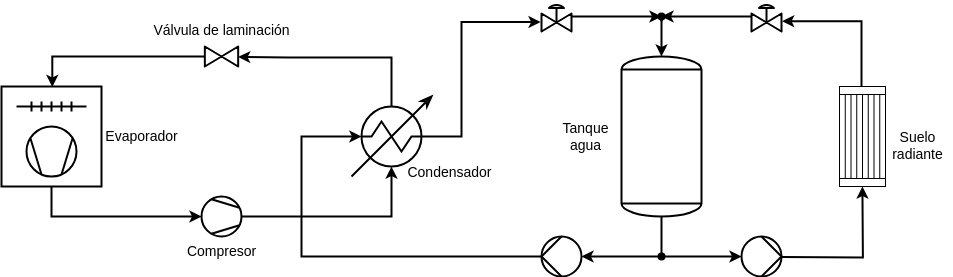
\includegraphics[width=1\textwidth]{./capitulos/resultados_discusion/images/sistema_termico.png}
	\caption{Diagrama térmico.}
	\label{fig:thermal_diagram}
\end{figure}

\subsection{Bomba de calor}

No hemos entrado a modelar la bomba de calor compuesta por evaporador,
compresor, condensador y válvula de laminación.

En su lugar hemos aproximado el COP (Coefficient of Performance) con los datos
encontrados en hojas técnicas para hacerlo función de la temperatura de salida
del agua, variable que hemos llamado $T_{cond}$, correspondiendo a la
temperatura de salida del condensador.

En una de las bombas de calor encontradas
\footnote{\url{https://www.daikin.es/content/dam/DACS/document-library/Pdfs-subidos-2022/Monobloc\%20EBLA\%209-11\%20-\%2014-16.pdf}}
se especifica un COP de 4.8 para una temperatura de 35ºC, y de 3.4 para 55ºC.
Así que se considera que el COP varía linealmente entre esos dos puntos, con un
mínimo en 0, y en 4.8 el COP máximo.

La función por partes es

\begin{equation}
	\text{\text{cop}}(T) =
	\begin{cases}
		4.8,              & \text{si } T < 35ºC          \\[10pt]
		26.36 + -0.069 T, & \text{si } T_1 \leq T < 55ºC \\[10pt]
		0,                & \text{si } T \geq 103.5ºC
	\end{cases}
\end{equation}

que se muestra en la figura \ref{fig:heat_pump_cop}

\begin{figure}[h] \centering
	\centering
	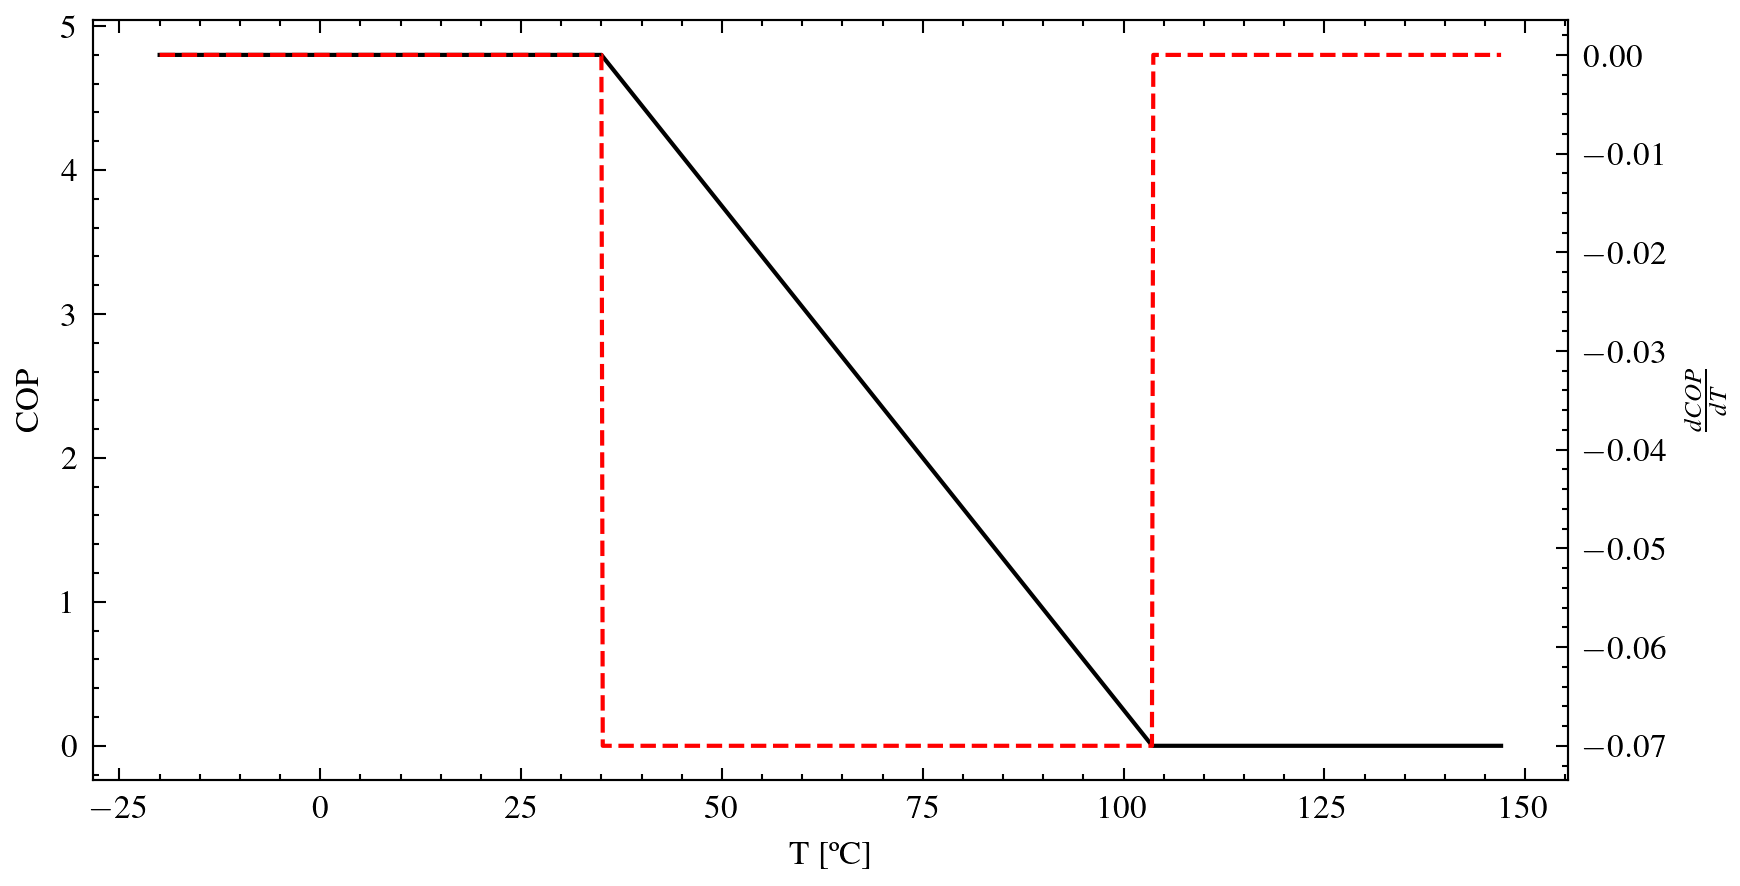
\includegraphics[width=1\textwidth]{./capitulos/resultados_discusion/images/heat_pump_cop.png}
	\caption{COP de la bomba de calor según la temperatura de salida del agua.}
	\label{fig:heat_pump_cop}
\end{figure}


\subsection{Tanque de agua}

Desde el tanque de agua aislado, tenemos dos flujos de entrada y salida
controlados por dos bombas de circulación. Un caudal para la bomba de calor
$\dot{m}_{cond}$, y otro para el suelo radiante $\dot{m}_{suelo}$.

La ecuación de conservación de la energía para el tanque con pérdidas de calor
por conducción con el ambiente (suponemos que se encuentra en el exterior de la
vivienda) es

\begin{align}
	\dot{m}_{\text{tanque}} & \cdot cp_{agua} \cdot \left( \frac{dT_{tanque}}{dt} \right) \nonumber \\
	                        & = \dot{m}_{cond} \cdot cp_{agua} \cdot T_{cond}  \nonumber            \\
	                        & + \dot{m}_{suelo} \cdot cp_{agua} \cdot T_{suelo} \nonumber           \\
	                        & - \dot{m}_{tanque} \cdot cp_{agua} \cdot T_{tanque} \nonumber         \\
	                        & - \dot{Q}_{perdida}
\end{align}

con las ecuaciones

\begin{align}
	\text{COP}        & = \text{cop}(T_{cond})                                         \\
	\dot{Q}_{cond}    & = \text{COP} \cdot P_{bomba}                                   \\
	\dot{Q}_{cond}    & = \dot{m}_{cond} \cdot cp_{agua} \cdot (T_{cond} - T_{tanque}) \\
	\dot{m}_{tanque}  & = \dot{m}_{cond} + \dot{m}_{suelo}                             \\
	\dot{Q}_{perdida} & = U_{tanque} \cdot A_{tanque} \cdot (T_{tanque} - T_{amb})
\end{align}

donde

\begin{itemize}
	\item $\text{COP}$: Coeficiente de rendimiento.
	\item $\text{cop}(T_{cond})$: Función que define el COP en función de $T_{cond}$.
	\item $m_{tanque}$: Masa del tanque.
	\item $cp_{agua}$: Calor específico del agua.
	\item $\dot{m}_{tanque}$: Flujo másico del tanque.
	\item $\dot{m}_{cond}$: Flujo másico del condensador.
	\item $\dot{m}_{suelo}$: Flujo másico del suelo radiante.
	\item $T_{tanque}$: Temperatura del tanque.
	\item $T_{cond}$: Temperatura a la salida el condensador.
	\item $T_{suelo}$: Temperatura a la salida del suelo radiante.
	\item $T_{amb}$: Temperatura ambiente.
	\item $\dot{Q}_{perdida}$: Pérdidas de calor por conducción.
	\item $\dot{Q}_{cond}$: Tasa de transferencia de calor en el condensador.
	\item $P_{bomba}$: Potencia del compresor.
	\item $U_{tanque}$: Coeficiente global de transferencia de calor del tanque.
	\item $A_{tanque}$: Área de la superficie del tanque.
\end{itemize}


\subsection{Suelo radiante}

Del tanque de agua hacemos circular una caudal de agua caliente por los
tubos del suelo radiante, que se encuentran incrustados en una losa de hormigón
sobre una superficie aislante.

Esta losa de hormigón que da una inercia térmica considerable al suelo, se ha
tomado de 5cm. Y tampoco hemos considerado que se haya recubierto la losa de
hormigón con ningún azulejo, porcelánico o madera.

\begin{figure}[h] \centering
	\centering
	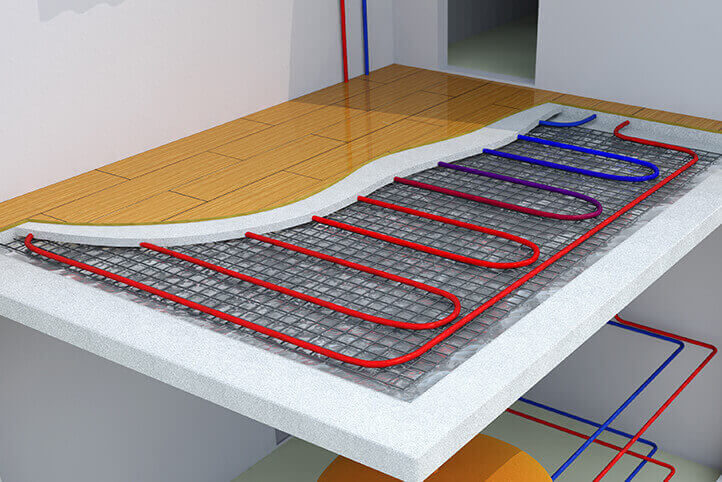
\includegraphics[width=1\textwidth]{./capitulos/resultados_discusion/images/radiant_heating_floor.jpg}
	\caption{Suelo radiante. Fuente: \url{https://www.palodurohardwoods.com/blog/radiant-heat/}}
	\label{fig:radiant_heating_floor}
\end{figure}

Este suelo calienta principalmente por radiación la habitación, y en menor
medida por convección natural, despreciándose el calor conducción.

De forma que el aire de la casa también tiene una inercia térmica, y pierde
calor por las paredes, tejado y ventanas.

Las ecuaciones del balance térmico del suelo y habitación por tanto también
están acopladas y son:
